% Provenance (never printed): NSI premiere "Architectures materielles: transmission de donnees dans un reseau,
% protocoles de communication, architecture d'un reseau" (bit alterne, adresses, masques, tables). See
% sources/book2/BRIEFS.md.
\chapter{Network Layers and Protocols}\label{ch:g11:network-protocols}

A message leaves a laptop, cut into packets. On its way it crosses a home network, a provider's network, a cable
under the sea and two more networks at the other end, and some of these lose a packet now and then. Yet the message
arrives whole, in order, and only once. No single network does this: each does one small job, and a few agreed rules,
stacked on one another, do the rest.

This chapter takes those rules apart: the \omterm{def:g11:network-protocols:layer}{layers} and the headers each one adds, the addresses and \omterm{def:g10:machine-integers:mask}{masks} that tell
which machines share a network, the tables that routers read to send a packet on, and a protocol that makes a
\omterm{def:g10:images-sound-compression:compression}{lossy} line reliable, which the weekend problem then pushes to its limit on a long cable.

\begin{omfigure}
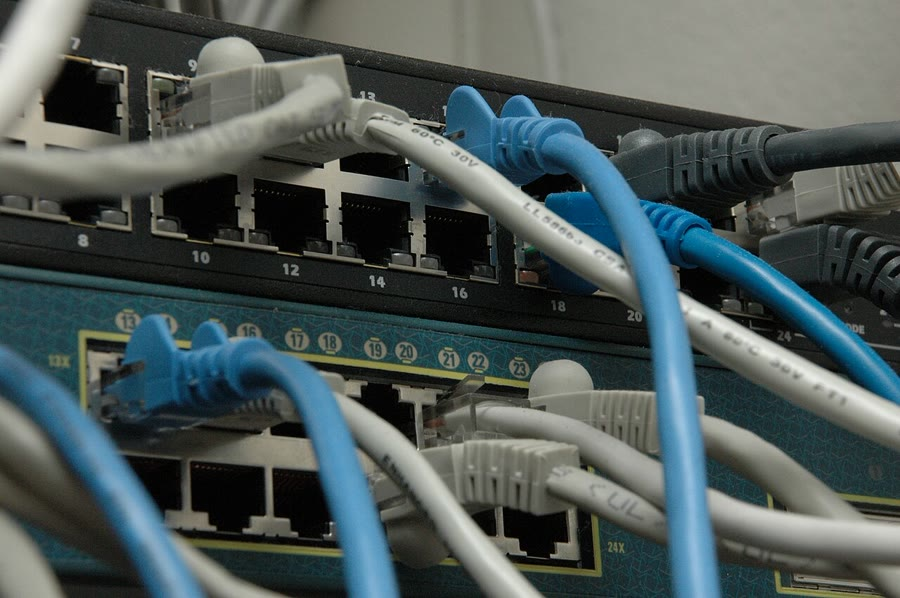
\includegraphics[width=0.5\linewidth]{images/book2/g11-network-switches.jpg}

{\small Two network switches with their cables plugged in: each cable joins one machine to the switch, which passes
each message on to the cable of its receiver. Photograph: ShakataGaNai, CC BY-SA 3.0.}
\end{omfigure}

\begin{recall}
Data crosses a network in packets, each with a packet header that holds, among other things, the addresses of its
sender and of its receiver. An IP address names a machine on the internet; routers pass packets from network to
network; the domain name system turns names into addresses; a client asks and a server answers (Book 1, grade 8).
\omterm{def:g10:http-clients-servers:http}{HTTP} is a protocol, and a \omterm{def:g10:http-clients-servers:port-number}{port number} names a program on a machine (chapter \ref{ch:g10:http-clients-servers}). A
\omterm{def:g10:machine-integers:mask}{mask} keeps some bits of a number with an AND (chapter \ref{ch:g10:machine-integers}).
\end{recall}

\section{Layers and headers}\label{sec:g11:network-protocols:layers}

A protocol fixes the format of the messages and the dialogue: who speaks first, what may answer what. \omterm{def:g10:http-clients-servers:http}{HTTP} is one,
but it says nothing of how its bytes cross the cable. That job is split among several protocols, stacked.

\begin{definition}[Layer, encapsulation]\label{def:g11:network-protocols:layer}
A network's protocols are organised in \emph{layers}\index{layer}, each using the service of the layer below and
offering one to the layer above: the \emph{application} layer (\omterm{def:g10:http-clients-servers:http}{HTTP}, for instance), the \emph{transport} layer, which
links two programs, the \emph{network} layer, which carries packets from machine to machine across networks, and
the \emph{link} layer, which carries frames across one cable or one radio link. Each layer adds its own header in
front of what it receives from above: this is \emph{encapsulation}\index{encapsulation}.
\end{definition}

\begin{omfigure}
\begin{tikzpicture}[font=\small, h/.style={draw, minimum height=7mm, fill=#1}, h/.default=white]
  \foreach \y/\n in {0/application, -1/transport, -2/network, -3/link} \node[anchor=east] at (-0.2,\y) {\n};
  \node[h=omMeth!12, minimum width=40mm, anchor=west] (d0) at (4.2,0) {data};
  \node[h=omDef!25, minimum width=14mm, anchor=west] at (2.8,-1) {T};
  \node[h=omMeth!12, minimum width=40mm, anchor=west] at (4.2,-1) {data};
  \node[h=omThm!20, minimum width=14mm, anchor=west] at (1.4,-2) {N};
  \node[h=omDef!25, minimum width=14mm, anchor=west] at (2.8,-2) {T};
  \node[h=omMeth!12, minimum width=40mm, anchor=west] at (4.2,-2) {data};
  \node[h=omProp!25, minimum width=14mm, anchor=west] at (0,-3) {L};
  \node[h=omThm!20, minimum width=14mm, anchor=west] at (1.4,-3) {N};
  \node[h=omDef!25, minimum width=14mm, anchor=west] at (2.8,-3) {T};
  \node[h=omMeth!12, minimum width=40mm, anchor=west] at (4.2,-3) {data};
  \draw[decorate, decoration={brace, amplitude=4pt, mirror}] (1.4,-3.45) -- node[below=4pt, font=\footnotesize]
    {the packet: the network layer's data unit} (8.2,-3.45);
\end{tikzpicture}

{\small \omterm{def:g11:network-protocols:layer}{Encapsulation}. Going down, each \omterm{def:g11:network-protocols:layer}{layer} puts its header (T, N, L) in front of what the \omterm{def:g11:network-protocols:layer}{layer} above gives it;
going up at the receiver, each \omterm{def:g11:network-protocols:layer}{layer} reads its own header and removes it.}
\end{omfigure}

The program below builds the three headers around an \omterm{def:g10:http-clients-servers:http}{HTTP} request. They are toy headers, cut down to the addresses
and \omterm{def:g10:http-clients-servers:port-number}{port numbers}; real ones hold more fields, as the next section shows.

\omcode{code/grade-11/04-network-protocols/listings/encapsulate.py}{1}{33}{Three \omterm{def:g11:network-protocols:layer}{layers} wrap a request, each in its
own header.}\label{lst:g11:network-protocols:encapsulate}

\omoutput{code/grade-11/04-network-protocols/outputs/encapsulate.txt}{Each line shows a header in hexadecimal and the
size of what it wraps. \code{c0 00 00 50} are the ports $49152$ and $80$; \code{c0 00 02 0a} is
\code{192.0.2.10}.}\label{out:g11:network-protocols:encapsulate}

A router opens the frame, reads the network header to choose where the packet goes next, and puts it in a new frame
for the next link: the link header changes at each step, the network header travels from end to end, and the
transport header is read only by the two machines at the ends.

\section{Addresses and the network mask}\label{sec:g11:network-protocols:addresses}

An IP address of the version used here, IPv4, has $32$ bits, written as four bytes in decimal separated by dots:
\code{192.0.2.10} is $11000000\ 00000000\ 00000010\ 00001010$. Its first bits name a network, the rest a machine in
that network.

\begin{definition}[Network mask, prefix]\label{def:g11:network-protocols:ip-address}
The \emph{network mask}\index{network mask} of a network is a $32$-bit number made of ones followed by zeros: the
bits under the ones are the network part of each address, the others the machine's part. The number $n$ of ones is
the \emph{prefix}\index{prefix} length, written after a slash: \code{192.0.2.0/24} is the network whose addresses share
their first $24$ bits with \code{192.0.2.0}. Two machines are on the same network when the AND of their address with
the \omterm{def:g10:machine-integers:mask}{mask} gives the same result.
\end{definition}
% ledger: g11:cidr-4632

The addresses in this chapter's examples come from three blocks set aside for documentation, \code{192.0.2.0/24},
\code{198.51.100.0/24} and \code{203.0.113.0/24}, which no real machine uses. Homes and schools use other reserved
blocks inside their own networks, such as \code{192.168.0.0/16} and \code{10.0.0.0/8}, which never appear on the
internet itself.
% ledger: g11:doc-5737
% ledger: g11:private-1918

\omoutput{code/grade-11/04-network-protocols/outputs/same_network.txt}{Python's \code{ipaddress} module knows \omterm{def:g10:machine-integers:mask}{masks}
and \omterm{def:g11:network-protocols:ip-address}{prefixes}. A /26 leaves $6$ bits to the machines: $2^6 = 64$
addresses.}\label{out:g11:network-protocols:same-network}

\omcode{code/grade-11/04-network-protocols/listings/mask_bits.py}{1}{23}{The network part by hand: a \omterm{def:g10:machine-integers:mask}{mask} built from
the \omterm{def:g11:network-protocols:ip-address}{prefix}, then an AND.}\label{lst:g11:network-protocols:mask-bits}

\omoutput{code/grade-11/04-network-protocols/outputs/mask_bits.txt}{The AND keeps the first $26$ bits and clears the
others; the module agrees.}\label{out:g11:network-protocols:mask-bits}

The first address of a network, all machine bits $0$, names the network itself, and the last, all machine bits $1$,
is used to reach every machine of the network at once: a /26 leaves $62$ addresses for machines.

\begin{omfigure}
\begin{bytefield}[bitwidth=1.08em]{32}
  \bitheader{0,4,8,16,19,24,31} \\
  \bitbox{4}{\scriptsize version} & \bitbox{4}{\scriptsize length} & \bitbox{8}{\scriptsize service} &
  \bitbox{16}{\small total length} \\
  \bitbox{16}{\small identification} & \bitbox{3}{\scriptsize flags} & \bitbox{13}{\small fragment offset} \\
  \bitbox{8}{\small time to live} & \bitbox{8}{\small protocol} & \bitbox{16}{\small header checksum} \\
  \bitbox{32}{\small source address} \\
  \bitbox{32}{\small destination address}
\end{bytefield}

{\small The header of an IPv4 packet, $32$ bits per row, $20$ bytes without options. Each router lowers the time to
live by one and drops the packet at zero, so a packet lost in a loop does not travel for ever.}
\end{omfigure}
% ledger: g11:ipv4-791

Thirty-two bits give about four billion addresses, too few for every device in the world. The newer version, IPv6,
uses $128$-bit addresses, written in hexadecimal; both versions run side by side on the internet.
% ledger: g11:ipv6-8200

\section{A routing table read by hand}\label{sec:g11:network-protocols:routing}

\begin{definition}[Routing table, next hop, default route]\label{def:g11:network-protocols:routing-table}
A router's \emph{routing table}\index{routing table} lists networks, each written with its \omterm{def:g11:network-protocols:ip-address}{prefix}, and for each the
\emph{next hop}\index{next hop}: the neighbouring router to pass the packet to, or ``direct'' when the network is
connected to the router itself. When several lines contain the destination, the router takes the one with the
longest \omterm{def:g11:network-protocols:ip-address}{prefix}, the most precise. The line \code{0.0.0.0/0}, which contains every address, is the \emph{default
route}\index{default route}: it is used when no other line fits.
\end{definition}

\begin{omfigure}
\begin{tikzpicture}[font=\small, r/.style={circle, draw, thick, fill=omDef!12, minimum size=8mm},
    n/.style={draw, rounded corners=3pt, fill=omMeth!10, align=center, font=\footnotesize}]
  \node[r] (A) at (0,0) {A};
  \node[r] (B) at (2.4,1.3) {B};
  \node[r] (C) at (2.4,-0.2) {C};
  \node[r] (D) at (2.4,-1.6) {D};
  \node[n] (h) at (-2.6,0) {\code{192.0.2.0/24}\\the school};
  \node[n] (nb) at (5.3,1.3) {\code{198.51.100.0/25}};
  \node[n] (nc) at (5.3,-0.2) {\code{198.51.100.128/25}};
  \node[n] (nd) at (5.3,-1.6) {the rest of\\the internet};
  \draw[thick] (h) -- node[above, font=\scriptsize] {port 1} (A) (A) -- (B) (A) -- (C) (A) -- (D);
  \draw[thick] (B) -- (nb) (C) -- (nc) (D) -- (nd);
  \node[anchor=north, font=\footnotesize] at (1.2,-2.3) {
    \begin{tabular}{ll}
      \multicolumn{2}{l}{\textbf{table of router A}} \\ \hline
      \code{192.0.2.0/24} & direct, port 1 \\
      \code{198.51.100.0/24} & B \\
      \code{198.51.100.128/25} & C \\
      \code{0.0.0.0/0} & D (default)
    \end{tabular}};
\end{tikzpicture}

{\small Router A and its table. The /24 line through B also contains the addresses of C's network; for those, the /25
line through C is longer, so it wins.}
\end{omfigure}

\omcode{code/grade-11/04-network-protocols/listings/route_lookup.py}{1}{24}{Router A's table, and the longest \omterm{def:g11:network-protocols:ip-address}{prefix}
match.}\label{lst:g11:network-protocols:route-lookup}

\omoutput{code/grade-11/04-network-protocols/outputs/route_lookup.txt}{Two lines contain \code{198.51.100.200}; the
/25 is longer. Nothing but the \omterm{def:g11:network-protocols:routing-table}{default route} contains
\code{203.0.113.5}.}\label{out:g11:network-protocols:route-lookup}

Each router decides only the \omterm{def:g11:network-protocols:routing-table}{next hop}. The packet's whole route is never written anywhere: it is the chain of these
local choices, which is why the tables of neighbouring routers must agree, and why routers exchange what they know
with one another.

\section{Reliable delivery over an unreliable network}\label{sec:g11:network-protocols:reliable}

Packets get lost: a router whose queue is full drops what arrives, a radio link loses a frame to noise. The network
\omterm{def:g11:network-protocols:layer}{layer} does not repair this. The two ends repair it themselves.

\begin{definition}[Acknowledgement, timeout, retransmission]\label{def:g11:network-protocols:ack}
An \emph{acknowledgement}\index{acknowledgement} is a short message by which the receiver tells the sender that a
packet arrived. If no acknowledgement comes back within a set time, the \emph{timeout}\index{timeout}, the sender
sends the packet again: a \emph{retransmission}\index{retransmission}.
\end{definition}

\omterm{def:g11:network-protocols:ack}{Retransmission} brings a new trap. If the packet arrived but its \omterm{def:g11:network-protocols:ack}{acknowledgement} was lost, the sender sends it again
and the receiver gets it twice. The receiver must tell a new packet from a copy.

\begin{definition}[Alternating-bit protocol]\label{def:g11:network-protocols:alternating-bit}
In the \emph{alternating-bit protocol}\index{alternating-bit protocol}, each packet carries one bit, $0$ for the first,
$1$ for the next, $0$ again, and so on. The sender sends a packet until an \omterm{def:g11:network-protocols:ack}{acknowledgement} with its bit comes back,
then moves to the next packet with the other bit. The receiver acknowledges every packet with the bit it carries, and
keeps it only if its bit is the one expected; a packet with the other bit is a copy, and is dropped.
\end{definition}

\begin{history}[A note of two pages]
The \omterm{def:g11:network-protocols:alternating-bit}{alternating-bit protocol} was published in May 1969 by K.~A.~Bartlett, R.~A.~Scantlebury and P.~T.~Wilkinson, in
a note of two pages on reliable transmission over links that lose messages.
% ledger: g11:abp-1969
\end{history}

The simulation below uses a channel that loses each item with a set probability, drawn from a seeded generator, so
that every run loses the same packets.

\omcode{code/grade-11/04-network-protocols/listings/lossy_channel.py}{1}{12}{A \omterm{def:g10:images-sound-compression:compression}{lossy} channel, reproducible thanks to its
seed.}\label{lst:g11:network-protocols:lossy-channel}

\omcode{code/grade-11/04-network-protocols/listings/alternating_bit.py}{1}{35}{The \omterm{def:g11:network-protocols:alternating-bit}{alternating-bit protocol}: the
sender's loop and the receiver's test.}\label{lst:g11:network-protocols:alternating-bit}

\omoutput{code/grade-11/04-network-protocols/outputs/alternating_bit.txt}{A lost \omterm{def:g11:network-protocols:ack}{acknowledgement} makes a copy, which the
receiver drops; a lost packet is simply sent again. Four messages arrive, once each, in
order.}\label{out:g11:network-protocols:alternating-bit}

\begin{omfigure}
\begin{tikzpicture}[font=\footnotesize, m/.style={->, thick, omThm}, k/.style={->, thick, omDef}]
  \node at (0,0.4) {sender}; \node at (5,0.4) {receiver};
  \draw[thick] (0,0) -- (0,-7.4); \draw[thick] (5,0) -- (5,-7.4);
  \draw[m] (0,-0.2) -- node[above, sloped] {$(0, a)$} (5,-0.9);
  \node[right] at (5,-0.9) {kept};
  \draw[k] (5,-1.0) -- node[below, sloped] {ack $0$} (3.0,-1.3);
  \node[text=omThm, font=\small\bfseries] at (2.9,-1.32) {$\times$};
  \node[left] at (0,-2.0) {timeout};
  \draw[m] (0,-2.0) -- node[above, sloped] {$(0, a)$} (5,-2.7);
  \node[right] at (5,-2.7) {copy, dropped};
  \draw[k] (5,-2.8) -- node[above, sloped] {ack $0$} (0,-3.5);
  \draw[m] (0,-4.1) -- node[above, sloped] {$(1, b)$} (2.2,-4.4);
  \node[text=omThm, font=\small\bfseries] at (2.3,-4.42) {$\times$};
  \node[left] at (0,-5.5) {timeout};
  \draw[m] (0,-5.5) -- node[above, sloped] {$(1, b)$} (5,-6.2);
  \node[right] at (5,-6.2) {kept};
  \draw[k] (5,-6.3) -- node[above, sloped] {ack $1$} (0,-7.0);
  \node[left] at (0,-7.0) {next: $(0, c)$};
\end{tikzpicture}

{\small Time flows downwards; a $\times$ marks a loss. A lost \omterm{def:g11:network-protocols:ack}{acknowledgement} (top) and a lost packet (middle): in both cases
the sender's \omterm{def:g11:network-protocols:ack}{timeout} sends the packet again, and the bit lets the receiver drop the copy.}
\end{omfigure}

Waiting for each \omterm{def:g11:network-protocols:ack}{acknowledgement} before sending on, \emph{stop and wait}, has a cost: while the packet and its
\omterm{def:g11:network-protocols:ack}{acknowledgement} travel, the line is idle. If sending a packet takes a time $T$ and the round trip a time $R$, the line
is busy a fraction $T / (T + R)$ of the time.

\omcode{code/grade-11/04-network-protocols/listings/throughput.py}{1}{15}{The share of time stop and wait keeps the line
busy.}\label{lst:g11:network-protocols:throughput}

\omoutput{code/grade-11/04-network-protocols/outputs/throughput.txt}{On long links stop and wait wastes almost all the
line. A ten times faster line does not help: the round trip is the
limit.}\label{out:g11:network-protocols:throughput}

\section{Ports and the transport layer}\label{sec:g11:network-protocols:transport}

An IP address names a machine; a \omterm{def:g10:http-clients-servers:port-number}{port number}, $16$ bits, names a program on it. Ports $0$ to $1023$ are the system
ports, given to well-known services, such as $80$ for \omterm{def:g10:http-clients-servers:http}{HTTP} and $443$ for \omterm{def:g10:http-clients-servers:https}{HTTPS}; a client's own port is usually taken
from the top of the range, $49152$ to $65535$, as in the frame of the first section.
% ledger: g11:ports-6335
% ledger: g10:http-ports

\begin{definition}[TCP, UDP]\label{def:g11:network-protocols:tcp-udp}
The internet's two main transport protocols are \emph{TCP}\index{TCP}, which gives two programs a reliable stream of
bytes, in order and without copies, by numbering the bytes, acknowledging them and sending again what is lost, and
\emph{UDP}\index{UDP}, which sends single datagrams with no \omterm{def:g11:network-protocols:ack}{acknowledgement}, so that they may be lost, duplicated or
arrive out of order. A TCP header has at least $20$ bytes, a UDP header $8$.
\end{definition}
% ledger: g11:tcp-9293
% ledger: g11:udp-768

\omterm{def:g11:network-protocols:tcp-udp}{TCP}'s reliability has a price in time, since a lost packet waits for its \omterm{def:g11:network-protocols:ack}{retransmission} and the bytes behind it wait
too. A video call prefers \omterm{def:g11:network-protocols:tcp-udp}{UDP}: a lost image is better skipped than shown late. Neither protocol promises when data
arrives; reliable does not mean fast.

\begin{definition}[Peer-to-peer network]\label{def:g11:network-protocols:p2p}
In a \emph{peer-to-peer network}\index{peer-to-peer network}, every machine is both client and server: each asks the
others for data and serves what it has, with no central server.
\end{definition}

Before a program can send anything to \code{library.example}, the name must become an address. A machine first looks
in a small local table, then, if the name is not there, asks the domain name system. The names ending in
\code{.example} are reserved for examples like this one.
% ledger: g11:example-tld

\omcode{code/grade-11/04-network-protocols/listings/hosts_lookup.py}{1}{23}{A local table of names, in the format of
the \omterm{def:g10:http-clients-servers:url}{hosts} file most systems keep.}\label{lst:g11:network-protocols:hosts}

\omoutput{code/grade-11/04-network-protocols/outputs/hosts_lookup.txt}{Two names are found locally; the third would go
to the name system.}\label{out:g11:network-protocols:hosts}

\section{Exercises}\label{sec:g11:network-protocols:exercises}

\begin{exercise}[$\star$]\label{exo:g11:network-protocols:1}
Give the network address of \code{192.168.10.37/24}.
\end{exercise}

\begin{exercise}[$\star$]\label{exo:g11:network-protocols:2}
How many addresses does a /26 network contain? How many machines can it hold, the first and last addresses set
apart?
\end{exercise}

\begin{exercise}[$\star$]\label{exo:g11:network-protocols:3}
With router A's table, where does a packet for \code{198.51.100.130} go? For \code{198.51.100.127}?
\end{exercise}

\begin{exercise}[$\star$]\label{exo:g11:network-protocols:4}
In what order do the headers come in a frame, from its first byte? Which of them does a router read and replace?
\end{exercise}

\begin{exercise}[$\star$]\label{exo:g11:network-protocols:5}
Write a function \code{same_network(a, b, prefix)} that tells whether two addresses, given as dotted strings, are on
the same network, without the \code{ipaddress} module's networks: build the \omterm{def:g10:machine-integers:mask}{mask}, then compare.
\end{exercise}

\begin{exercise}[$\star\star$]\label{exo:g11:network-protocols:6}
A student computes the network part of \code{192.0.2.37/26} with an OR instead of an AND, and gets
\code{255.255.255.229}. Explain what the OR did, bit by bit.
\end{exercise}

\begin{exercise}[$\star\star$]\label{exo:g11:network-protocols:7}
Write a function \code{lookup(table, address)} that takes a table as a list of pairs, \omterm{def:g11:network-protocols:ip-address}{prefix} and \omterm{def:g11:network-protocols:routing-table}{next hop}, and
returns the \omterm{def:g11:network-protocols:routing-table}{next hop} by longest \omterm{def:g11:network-protocols:ip-address}{prefix} match, or \code{None} if no line contains the address.
\end{exercise}

\begin{exercise}[$\star\star$]\label{exo:g11:network-protocols:8}
A program sends a message of $100$ bytes over \omterm{def:g11:network-protocols:tcp-udp}{TCP} and IPv4 on an Ethernet link, whose header has $14$ bytes:
two addresses of $6$ bytes and a type of $2$. How many bytes leave the machine, and what share of them are headers?
% ledger: g11:ethernet-894
\end{exercise}

\begin{exercise}[$\star\star$]\label{exo:g11:network-protocols:9}
The \omterm{def:g11:network-protocols:alternating-bit}{alternating-bit protocol} sends the messages \code{x} and \code{y}. The first packet sent is lost; the first
\omterm{def:g11:network-protocols:ack}{acknowledgement} of \code{y} is lost; nothing else is. Write the trace, in the format of the chapter's output, and count
the sends.
\end{exercise}

\begin{exercise}[$\star\star$]\label{exo:g11:network-protocols:10}
A receiver keeps every packet without checking its bit. Show, with a lost \omterm{def:g11:network-protocols:ack}{acknowledgement}, what goes wrong.
\end{exercise}

\begin{exercise}[$\star\star$]\label{exo:g11:network-protocols:11}
A line of $10$~Mbit/s sends packets of $1000$ bytes by stop and wait, with a round trip of $3.2$~ms. What share of the
time is the line busy, and what is the useful rate?
\end{exercise}

\begin{exercise}[$\star\star\star$]\label{exo:g11:network-protocols:12}
The channel may lose packets and \omterm{def:g11:network-protocols:ack}{acknowledgements}, but never reorders them and never invents them. Show that the
receiver of the \omterm{def:g11:network-protocols:alternating-bit}{alternating-bit protocol} keeps every message exactly once, in order. Consider what the receiver may see
while the sender is sending one message.
\end{exercise}

\begin{exercise}[$\star\star\star$]\label{exo:g11:network-protocols:13}
With a window of $w$, the sender may have up to $w$ packets sent and not yet acknowledged. Write
\code{window_time(n, w, rtt)}: time is counted in ticks, one packet is sent per tick at most, and the \omterm{def:g11:network-protocols:ack}{acknowledgement}
of a packet sent at tick $t$ arrives at tick $t + 1 + \mathit{rtt}$. Return the tick at which the last \omterm{def:g11:network-protocols:ack}{acknowledgement}
arrives, with no loss. Compare $w = 1$, $2$ and $5$ for $n = 10$, $\mathit{rtt} = 4$.
\end{exercise}

\begin{exercise}[$\star\star\star$]\label{exo:g11:network-protocols:14}
Suppose now the channel may delay a packet and deliver it after later ones. Find a sequence of events where the
alternating-bit receiver keeps a message twice and loses another.
\end{exercise}

\begin{exercise}[$\star\star\star$]\label{exo:g11:network-protocols:15}
Split \code{192.0.2.0/24} into four networks of equal size. Give each one's \omterm{def:g11:network-protocols:ip-address}{prefix}, its first and last addresses, and
the number of machines it can hold.
\end{exercise}

\section{Problem: Stop and Wait Across the Sea}\label{sec:g11:network-protocols:problem}

\begin{problem}[{Weekend problem --- how many packets in flight fill a long line}]\label{pb:g11:network-protocols:1}
A cable of $6000$~km under the sea joins two cities. It carries $1$~Gbit/s, and its signals travel at
$200\,000$~km/s. Packets have $1500$ bytes. The \omterm{def:g11:network-protocols:ack}{acknowledgements} are so short that their own sending time is
neglected, and so is the time the machines take to answer. The program below computes what the line delivers when the
sender may have $w$ packets in flight before it must wait.

\omcode{code/grade-11/04-network-protocols/listings/sea_link.py}{1}{16}{The sea cable, with a window of $w$
packets.}\label{lst:g11:network-protocols:sea-link}

\omoutput{code/grade-11/04-network-protocols/outputs/sea_link.txt}{Busy share and useful rate for several
windows.}\label{out:g11:network-protocols:sea-link}

\medskip\noindent\textbf{Part I --- The line.}
\begin{enumerate}
  \item How long does the sender take to put one packet on the line?
  \item How long does a signal take to cross the cable one way? What is the round trip?
  \item Why may the \omterm{def:g11:network-protocols:ack}{acknowledgement}'s own sending time be neglected here?
  \item While the first bit crosses the cable, how many bits has the sender put behind it at full rate?
\end{enumerate}

\medskip\noindent\textbf{Part II --- Stop and wait.}
\begin{enumerate}[resume]
  \item With stop and wait, how long passes between the start of one packet and the start of the next?
  \item How many packets per second does this make, and what useful rate?
  \item How long would a file of $1$~GB, $8 \times 10^9$ bits, take to cross?
  \item Check your answers against the line \code{window 1} of the output.
\end{enumerate}

\medskip\noindent\textbf{Part III --- The busy share.}
\begin{enumerate}[resume]
  \item Explain the formula $T / (T + R)$ for stop and wait.
  \item Compute it here, as a percentage and as ``one in how many''.
  \item The line is replaced by one of $10$~Gbit/s. What happens to the busy share, and to the useful rate?
  \item Name two changes that would raise the useful rate of stop and wait, and say why neither helps much here.
\end{enumerate}

\medskip\noindent\textbf{Part IV --- The window.}
\begin{enumerate}[resume]
  \item Explain why, with a window of $w$, the busy share is the smaller of $1$ and $wT / (T + R)$.
  \item Check the line \code{window 1000} of the output by hand.
  \item Find the smallest window that keeps the line busy all the time, and check it against the program.
  \item How many bytes are in flight, sent and not yet acknowledged, at full rate? The sender must keep them all, in
    case it has to send them again: why?
  \item Why can the packets no longer carry a single bit, as in the \omterm{def:g11:network-protocols:alternating-bit}{alternating-bit protocol}?
  \item If the cable lost one packet in a thousand, about how many losses would happen per second at full rate?
  \item The window field of a \omterm{def:g11:network-protocols:tcp-udp}{TCP} header has $16$ bits and counts bytes; a larger window needs an extension that
    shifts it. Without that extension, how many full packets fit in the largest window, and what busy share would it
    allow on this cable?
% ledger: g11:tcp-window
  \item State the result: the busy share of stop and wait on this cable, and the window that fills it.
\end{enumerate}
\end{problem}
